\section{Research Plan} 
\label{sec:research}

% 30 pts for explanation here combined with timeline and timeline summary below
Re-state the problem you are trying to solve and then explain how you plan to
solve it. Is it designing a new visualization? Is it designing a new library?
Is it running a controlled experiment? Is it something else?

Note this is a {\em plan}. The plan may change as you make discoveries during
your project. However, you must describe what your plan is assuming everything
goes as expected. 

You should also describe what difficulties you are likely to encounter in the
various parts of your plans. Suggest alternative measures you could take
should those difficulties arise.

You may refer to other sections so as not to repeat yourself -- for example,
referencing \autoref{sec:background}.

You may want to use figures to illustrate your point, such as
\autoref{fig:sample}.

\begin{figure}[h]
 \centering % avoid the use of \begin{center}...\end{center} and use \centering instead (more compact)
 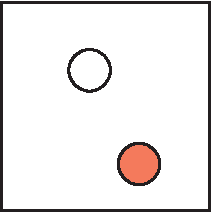
\includegraphics[width=1.5in]{figs/sample}
 \caption{Figure illustrating some proposed designs.}
 \label{fig:sample}
\end{figure}

% 5 pts
\subsection{Data}
\label{sec:data}

Describe the data here. Describe whether you already have access to the data
and if not, what is required to obtain the data. If you don't already have the
data, explain how long it will take to retrieve it. 

% 15 pts
\subsection{Evaluation}
\label{sec:eval}

Describe your plan for evaluating your work during this project. How will you
demonstrate that you have successfully solved the problem? How will you
validate the work you have produced?

Then, describe how you would evaluate the work beyond the timeframe of the
project. Without time constraints, what would you do? Do you have the
resources (people, time, equipment, data, money) to implement this plan in
the future? Does your plan for evaluating your work during the project serve
as a first step to this evaluation?

% 5 pts
\subsection{Technology}
\label{sec:tech}

Describe what technologies you intend to use (e.g., programming languages,
platforms, existing libraries) and why they make sense for your project. Do
they serve your users better than other technologies? Are you able to take
advantage of existing work/libraries for your domain with this technology
rather than HTML/CSS/JS and d3js?  

\subsection{Timeline}
\label{sec:timeline}

Adapt the milestones for the class project to the specifics of your project
and summarize in Table~\ref{tab:milestones}. Do not simply copy the current
text as is. Your milestones should be specific to your problem, the type of
project you have, and your plan.

The expectations are as follows:

\vspace{1.5ex}\noindent\textbf{Project Milestone Two} should include any task
and data abstraction necessary to support the project design whether it is
designing a user study, designing a new visualization, or designing a new
library. Initial designs should be included with discussion of the rationale
in support of the design. Data supporting all of these findings in terms of
background work or newly collected data (e.g., interviews, observations)
should be cited or discussed.

Additionally, the related works should be updated with a more thorough
literature review. Changes to the status of the data and the choices of
technology should be discussed.

If you are doing a literature review or a taxonomy, you should have a
preliminary list of papers you will review, along with an explanation of the
methodology you used to generate that list of papers (e.g., which venues did
you start with? which years? how did you follow citations?)

\vspace{1.5ex}\noindent\textbf{Project Milestone Three} should include the
results of the first chunk of work that needs to be done. In most projects
with implementation this will involve a working data reader and at least one visualization,
library feature, or study question type working. The milestone should include
images of these features and a discussion of what they do. The demonstration
should run with minimal effort and the code should be included in the
repository. For projects involving heavy literature review, this milestone
should include annotations and notes for half of the selected papers.
Including a preliminary schema will help me give you feedback.

In the corresponding report, discussion of project progress as well as any
revisions to the data, technology choice, and scope should be included.

\vspace{1.5ex}\noindent\textbf{Project Milestone Four} should include a
complete working prototype of the main project artifact, such as a
visualization tool, a visualization library, a working study with experimental
objects and stimuli complete, or completed literature annotations with an
categorization schema. The demonstration should run with minimal effort and
the code should be included in the repository.

In the corresponding report, discussion of project progress as well as any
revisions to the data, technology choice, and scope should be included. The
plan for evaluation especially should be updated indicating the plan for
milestone five and any preliminary work in the design of that evaluation.


\vspace{1.5ex}\noindent\textbf{Project Milestone Five} should include initial
evaluation of the work from project milestone four and recommendations for
improvement. Artifacts generated (e.g., pre-observation
plan, observation notes, data from studies) during this evaluation should be
included in the repository. Literature-based projects should include a
refinement of the findings from the previous milestone.



\begin{table}[h]
%% Table captions on top in journal version
 \caption{Project Milestones}\vspace{1ex} % the \vspace adds some space after the top caption
 \label{tab:milestones}
 \scriptsize
 \centering % avoid the use of \begin{center}...\end{center} and use \centering instead (more compact)
   \begin{tabular}{r|r}
     Milestone & Description (\%)\\
   \hline
     PM2 & Conduct interviews with hydrologists, sketch designs, \\
         & data and task abstractions written\\
     PM3 & Central (map) view of data working with basic pan and \\
         & zoom interactions, initial structure for multiple \\
	 & coordinated view\\
     PM4 & All views working including histogram selector and list \\
	 & view, advanced interactions added to map view, preliminary \\
	 & tasks selected for evaluation \\
     PM5 & Evaluation sessions with three hydrologists, data coded \\
         & and summarized.\\
   \end{tabular}
\end{table}

